%!TEX root = ../main.tex
\section{Simulation Experiments}
\label{sec:demoTechnology}
To demonstrate and analyze the capabilities of the control policy, we used an 80$ \times $80 m patch of terrain. The reduced scale of the test environment allowed for rapid evaluation and inclusion of tests using deformable terrain based on the Soil Contact Model (SCM) \cite{ChronoSCM2019}. For all tests, the vehicle is placed at world location (-35,35); to be successful, it must navigate safely to within a 10 m radius of world location (35,-35). This setup was a matter of convenience and is not a limitation of the policy. Since training used a larger patch of 120$ \times $120 m, it is important to note that parameters such as number of obstacles and height of terrain cannot be compared directly with testing; this was done on purpose. For the terrain patch, and equivalent number of obstacles to the 50 used in training is approximately 22. Additionally, the maximum height difference of 10 m in training is equivalent to a height of approximately 7.25 m on the testing terrain. Furthermore, in testing, to prevent the vehicle from successfully navigating purely along the diagonal straight toward the destination, five obstacles were placed randomly near the diagonal to force non-trivial trajectories. Overall, the tests were conducted with a higher-complexity environment that used in training. They were designed to probe the robustness of the algorithm and understand to what extent the policy could be used on never-before-seen terrain. We looked at ($i$) increased levels of hilliness; ($ii$) increased number of obstacles; and ($iii$) alterations of the soil including rigid, hard-deformable (silt-like), and soft-deformable (snow-like). 

Figure \ref{fig:scm_soft_hilly_deformed} shows a snapshot of one scenario: the soft deformable terrain used for testing robustness; a capture of the image from the camera sensor used by the NN; and the position of the vehicle along its current trajectory with the obstacles and height map overlaid for context (height map: black is valleys, white is peaks). 

\begin{figure}[h]
    \centering
    \includegraphics[height=.1095\paperheight]{images/demonstration/scm_soft_hilly_montage_final.png}
    \caption{Snapshot of a scenario used for testing. Left: third-person perspective of the vehicle; center: image from the camera's view at the resolution used in training 80$ \times $45 pixels; right: the current progress of the vehicle amount the hills and obstacles corresponding to the images on left. }
    \label{fig:scm_soft_hilly_deformed}
\end{figure}

Figure \ref{fig:example_paths} shows an example set of paths navigated by the Gator in the test environment. In Fig. \ref{fig:rigid_flat_3_example12}, the vehicle avoids a sparse environment, limited to 20 obstacles. By increasing the obstacles to 50, as shown in Fig. \ref{fig:rigid_flat_9_example22}, the complexity of the test environment forces the policy into a correspondingly complex path. An example failure is illustrated in Fig. \ref{fig:rigid_flat_9_failure_example0} where the vehicle does not reach the destination owing to a collision. Any scenario where the vehicle collides with an obstacle is deemed a failure, regardless of how directly the vehicle collides with the obstacle. The last example, shown in Fig. \ref{fig:rigid_height_map_example13}, demonstrates the vehicle navigating a hilly terrain, created from a programmatically generated random height map.


\begin{figure}[h]
    \captionsetup{justification=centering}
    \centering
    \begin{subfigure}{0.24\textwidth}
        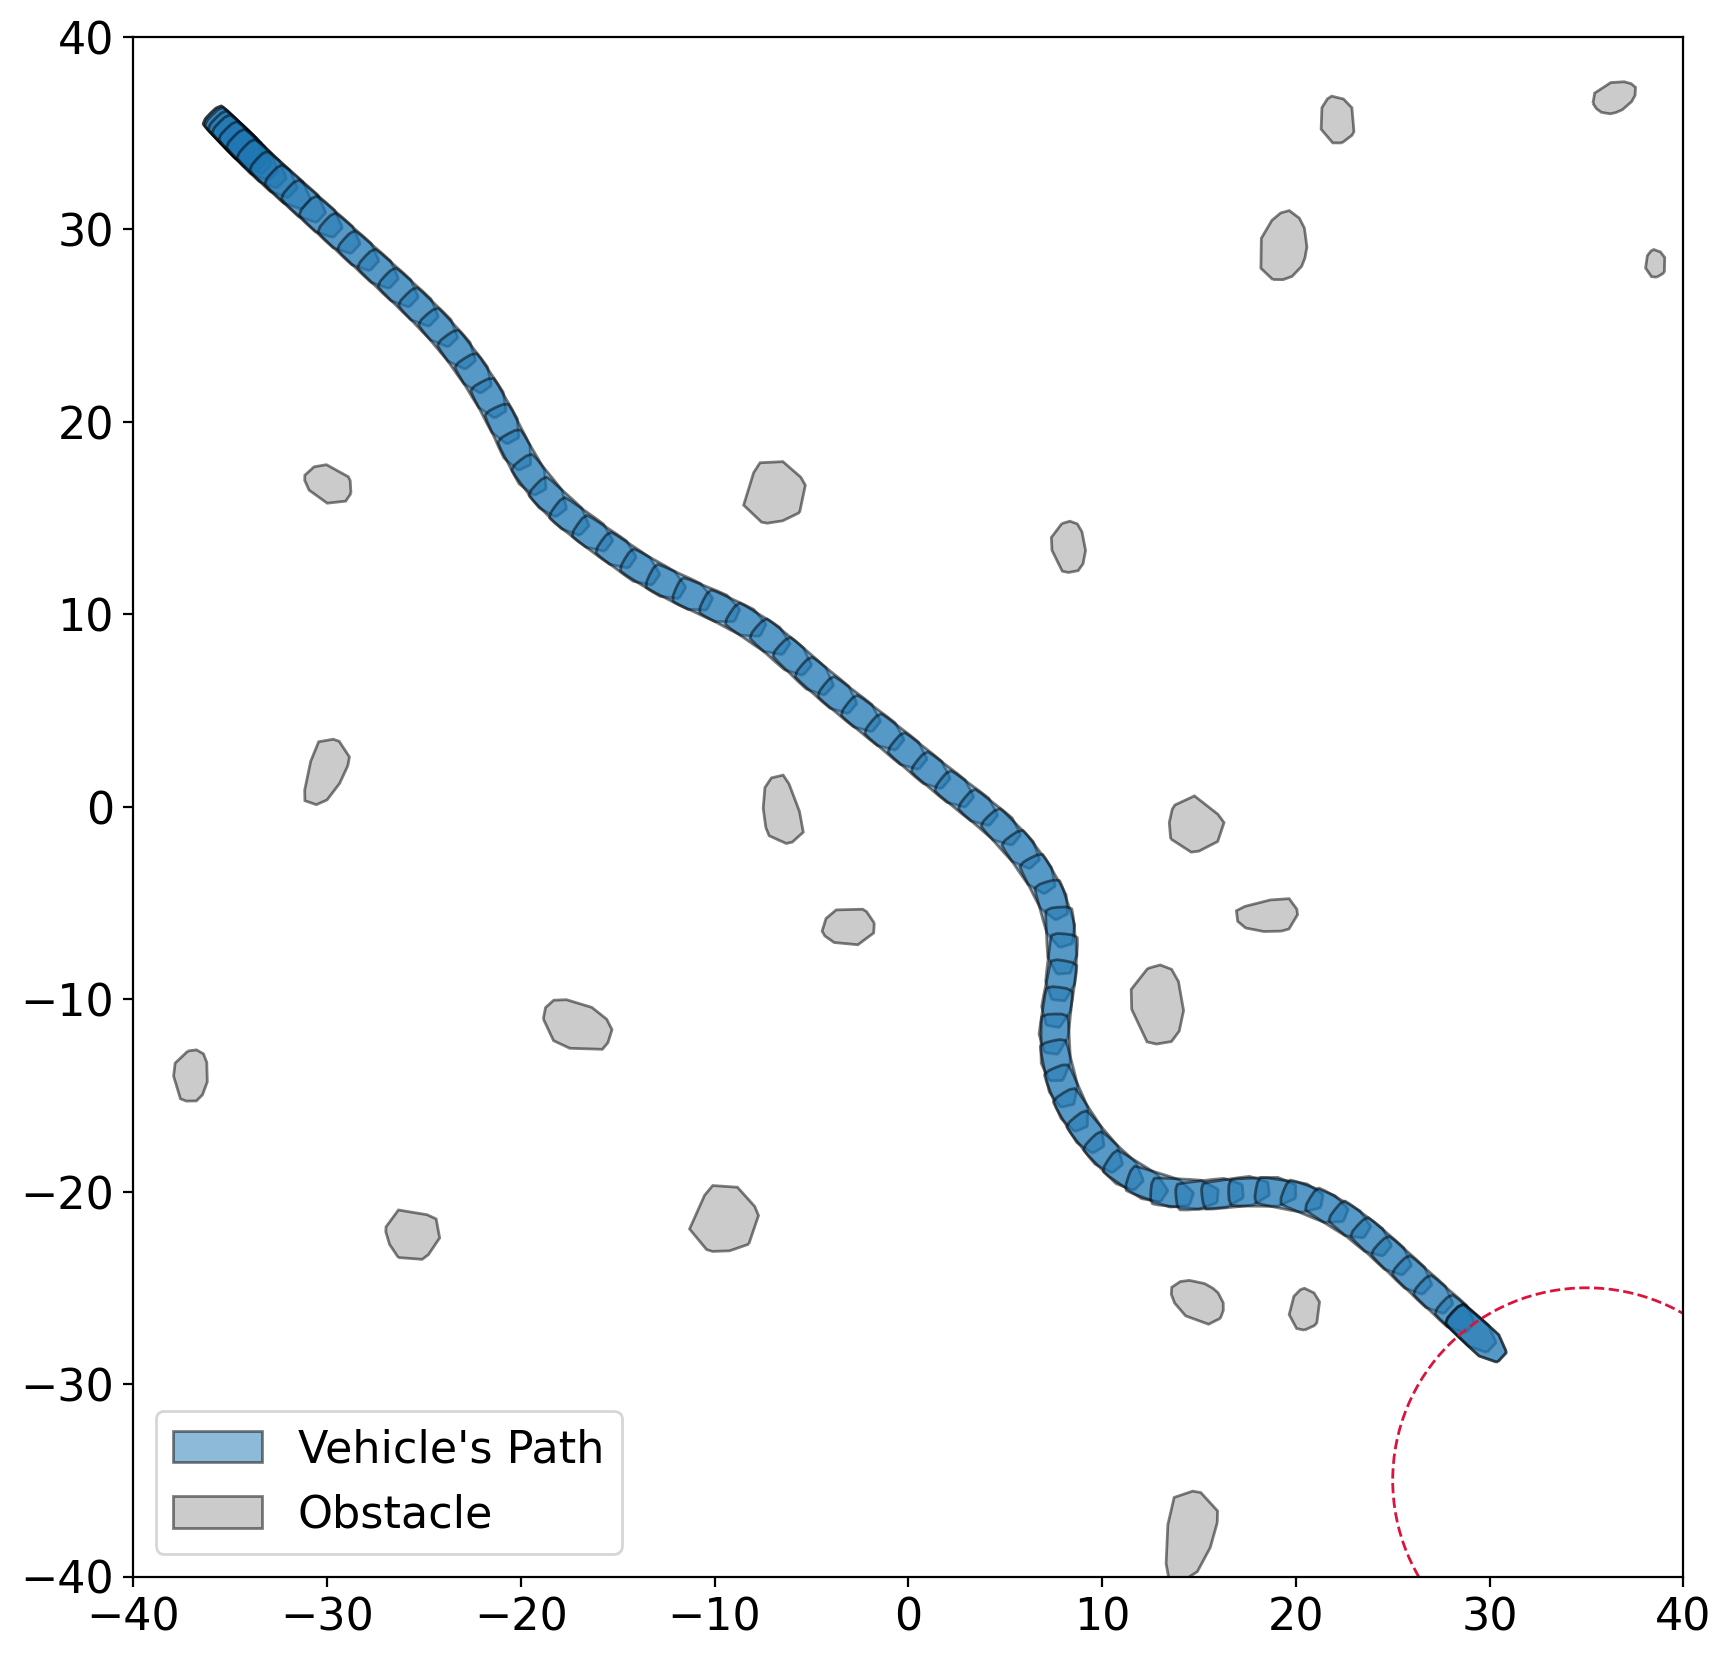
\includegraphics[height=.12\paperheight]{images/demonstration/rigid_flat_3_example12.png}
        \caption{}
        \label{fig:rigid_flat_3_example12}
    \end{subfigure}
    \hfill
    \begin{subfigure}{0.24\textwidth}
        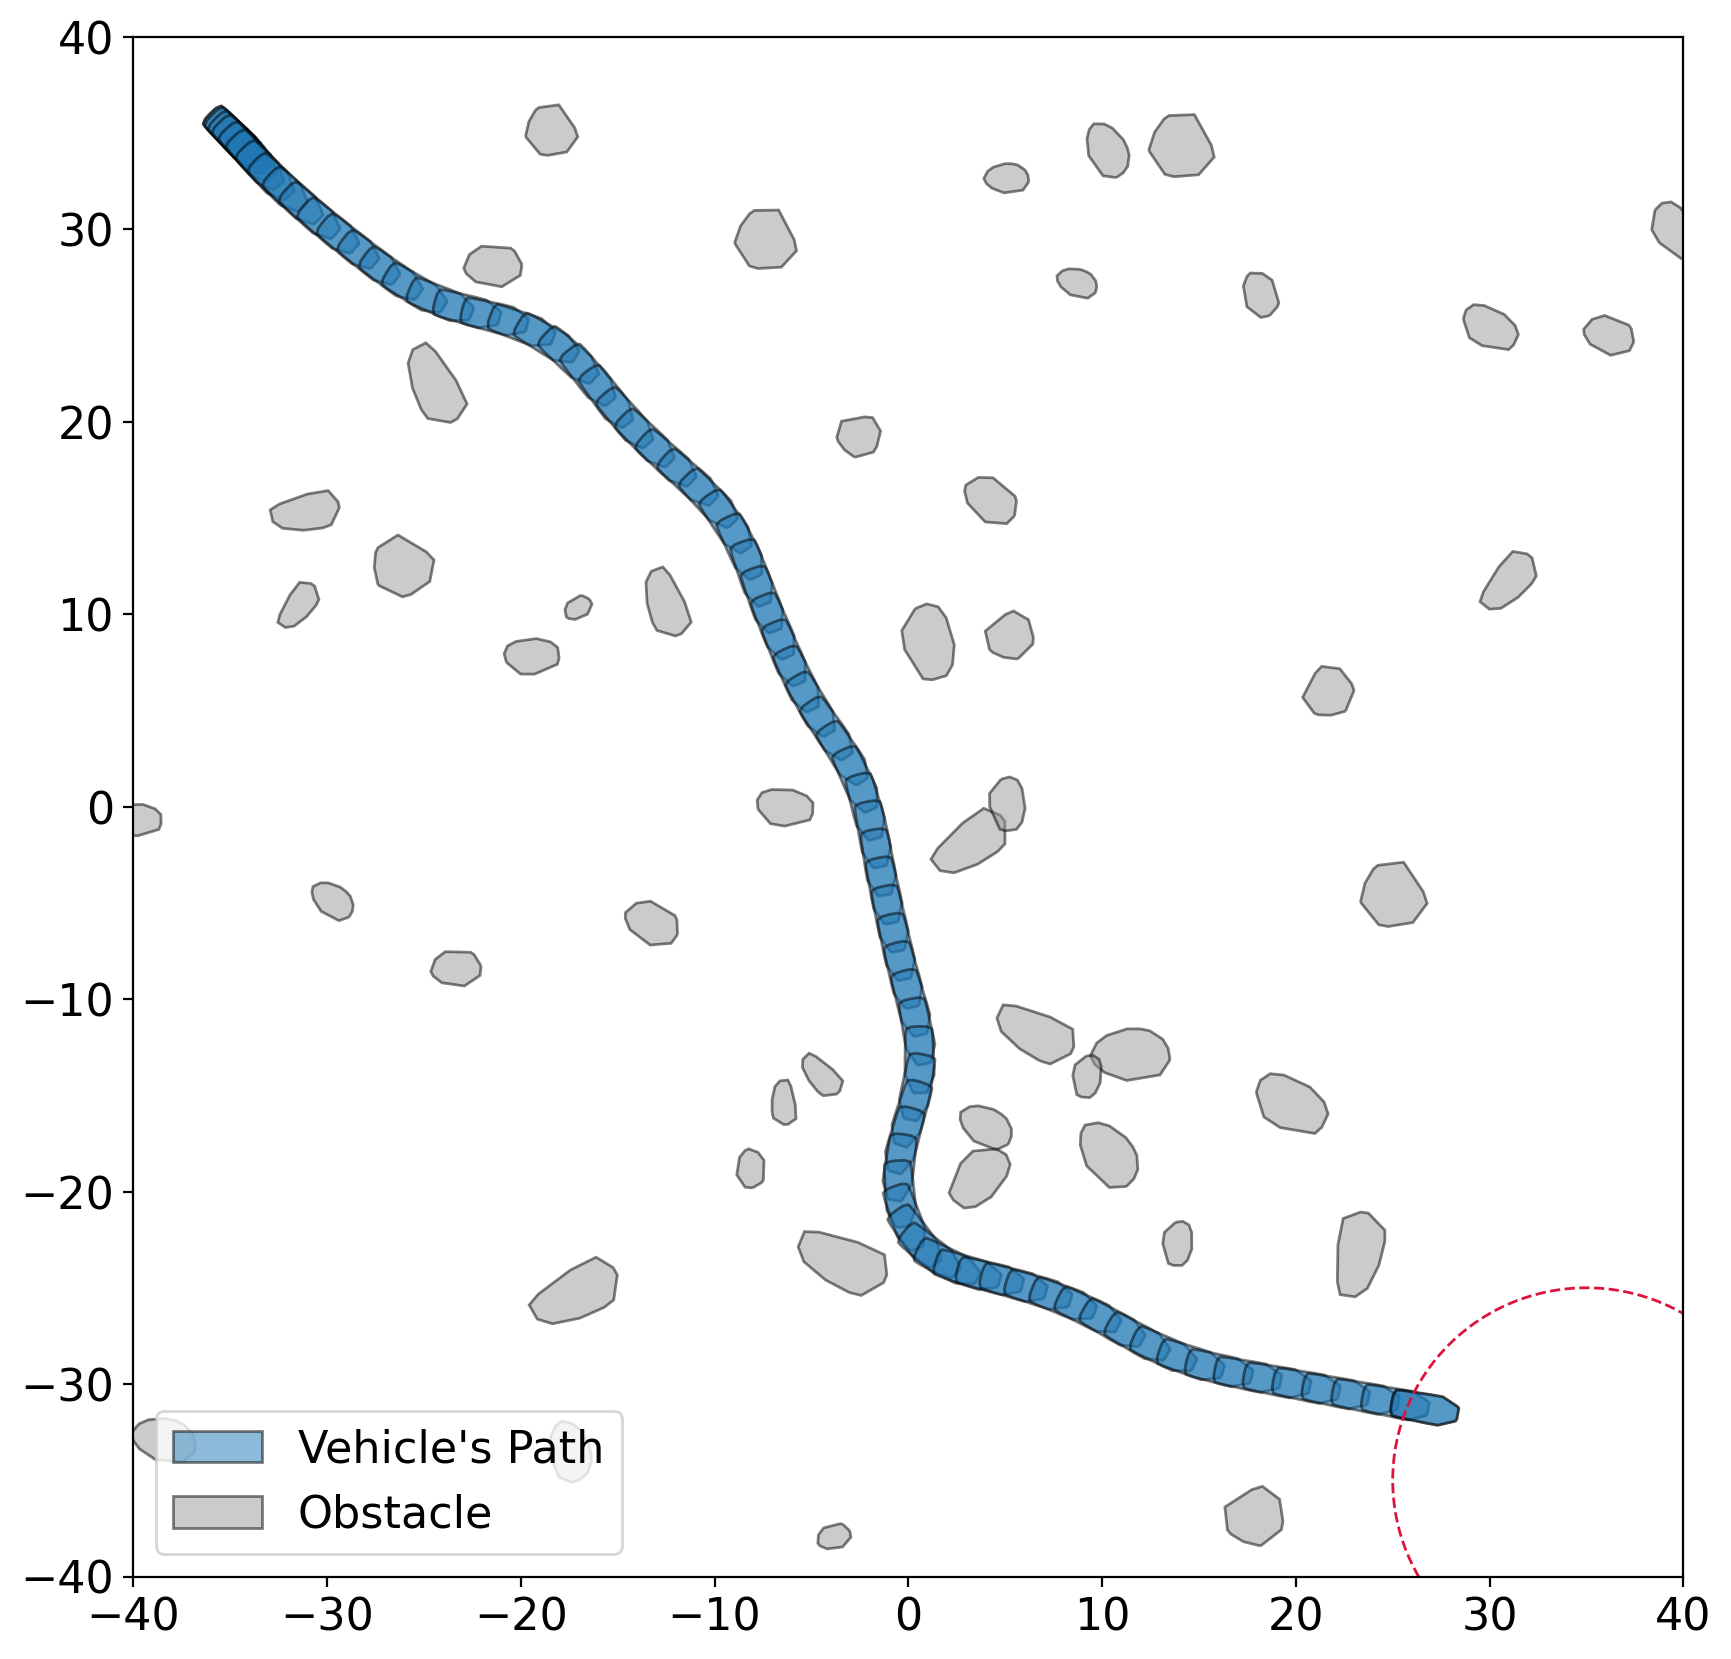
\includegraphics[height=.12\paperheight]{images/demonstration/rigid_flat_9_example22.png}
        \caption{}
        \label{fig:rigid_flat_9_example22}
    \end{subfigure}
    \hfill
    \begin{subfigure}{0.24\textwidth}
        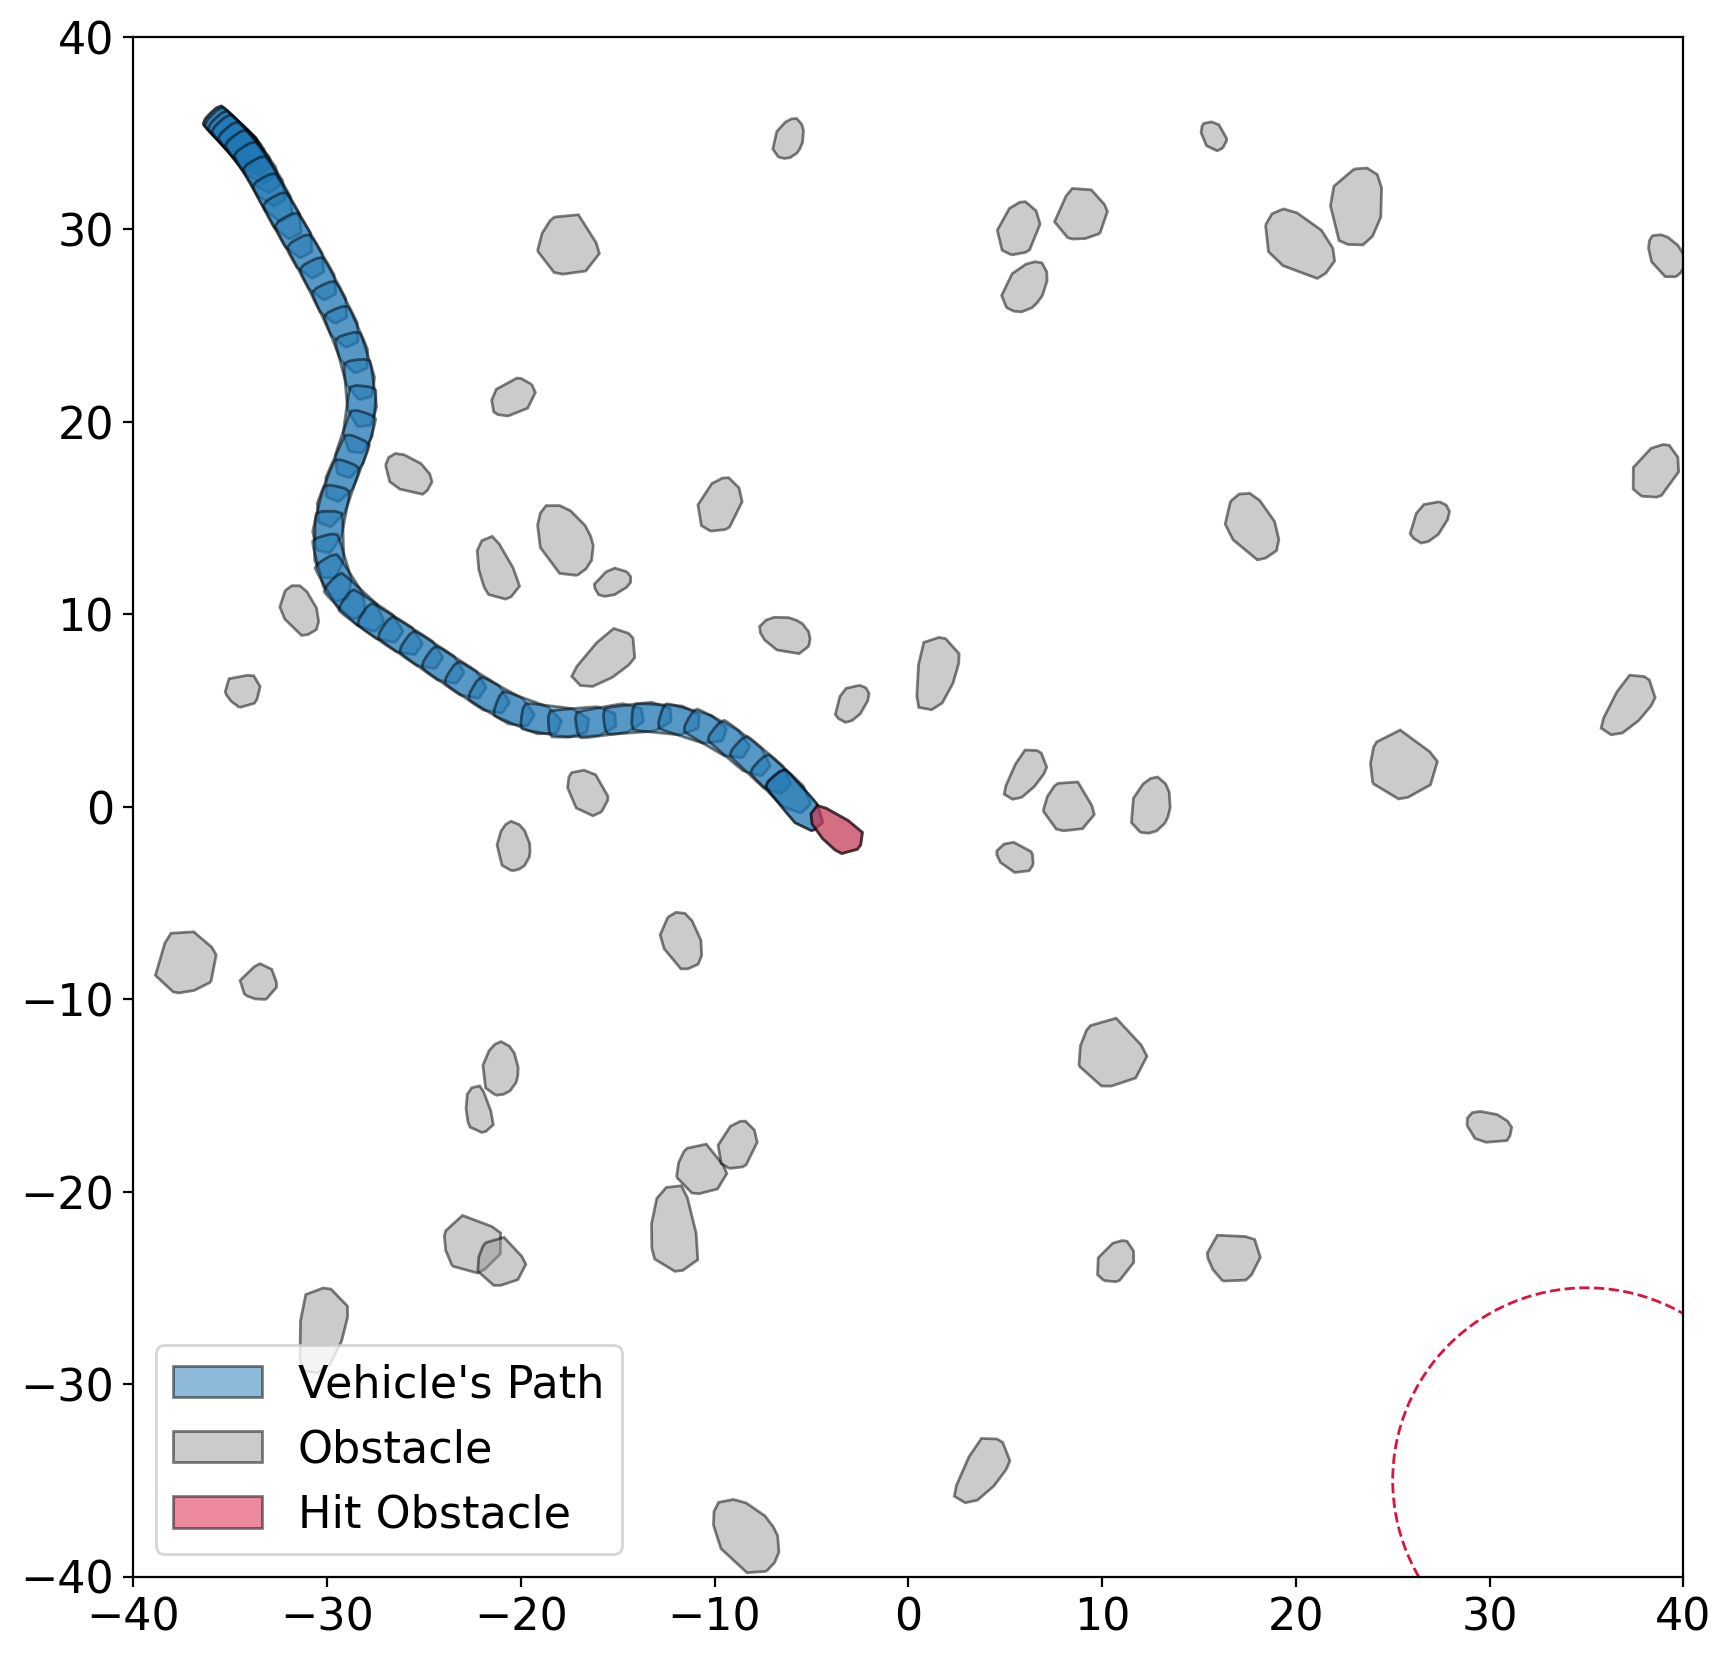
\includegraphics[height=.12\paperheight]{images/demonstration/rigid_flat_9_failure_example0.png}
        \caption{}
        \label{fig:rigid_flat_9_failure_example0}
    \end{subfigure}
    \hfill
    \begin{subfigure}{0.24\textwidth}
        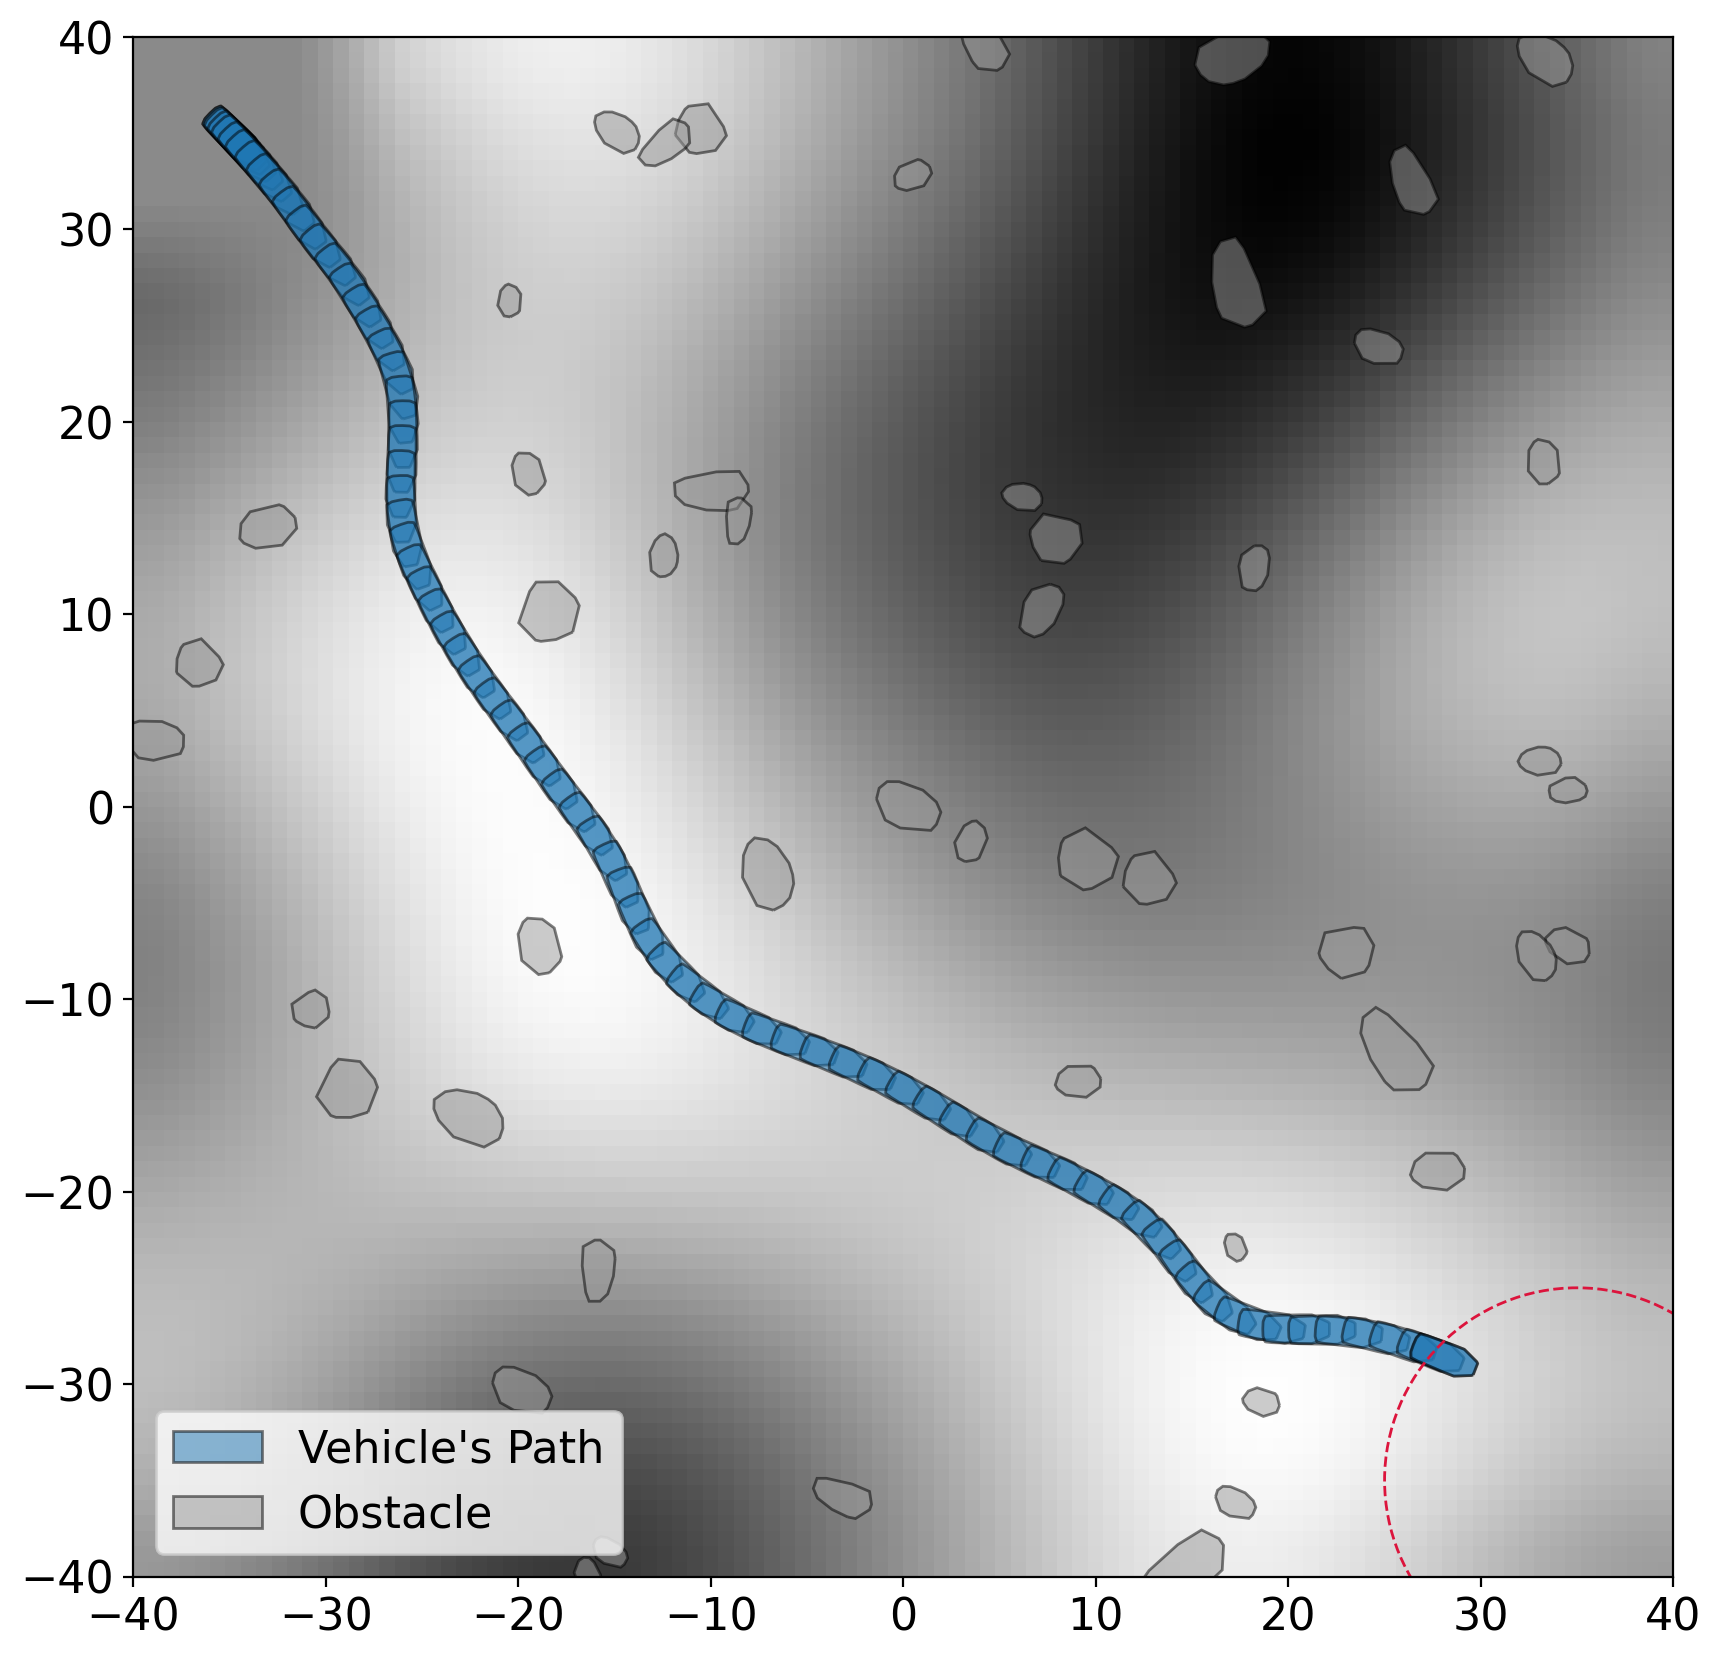
\includegraphics[height=.12\paperheight]{images/demonstration/rigid_height_map_example13.png}
        \caption{}
        \label{fig:rigid_height_map_example13}
    \end{subfigure}
    \caption{Example test scenarios: (a) 20 obstacles, (b) 50 obstacles, (c) failure with 50 obstacles, (d) hilly terrain with 50 obstacles.}
    \label{fig:example_paths}
\end{figure}

In an attempt to assess the practicality of the vehicle's chosen path, a Particle Swarm Optimization (PSO) algorithm \cite{PSOObstacleAvoidance} with global knowledge of the environment was used to generate reference trajectories in the environment; they were used in post-processing only, for comparison purposes. Figure \ref{fig:rigid_flat_pso_example3} shows a comparison between the trained vehicle's path and a trajectory generated using the PSO path planner. In this example, 40 obstacles are present on rigid, flat terrain. %What would have been undesirable to see was that the trained vehicle skirted the edges of the domain or assumed unreasonable trajectories. This turned out to not be the case.

\begin{figure}[h]
    \captionsetup{justification=centering}
    \centering
    \begin{subfigure}{0.329\textwidth}
        \centering
        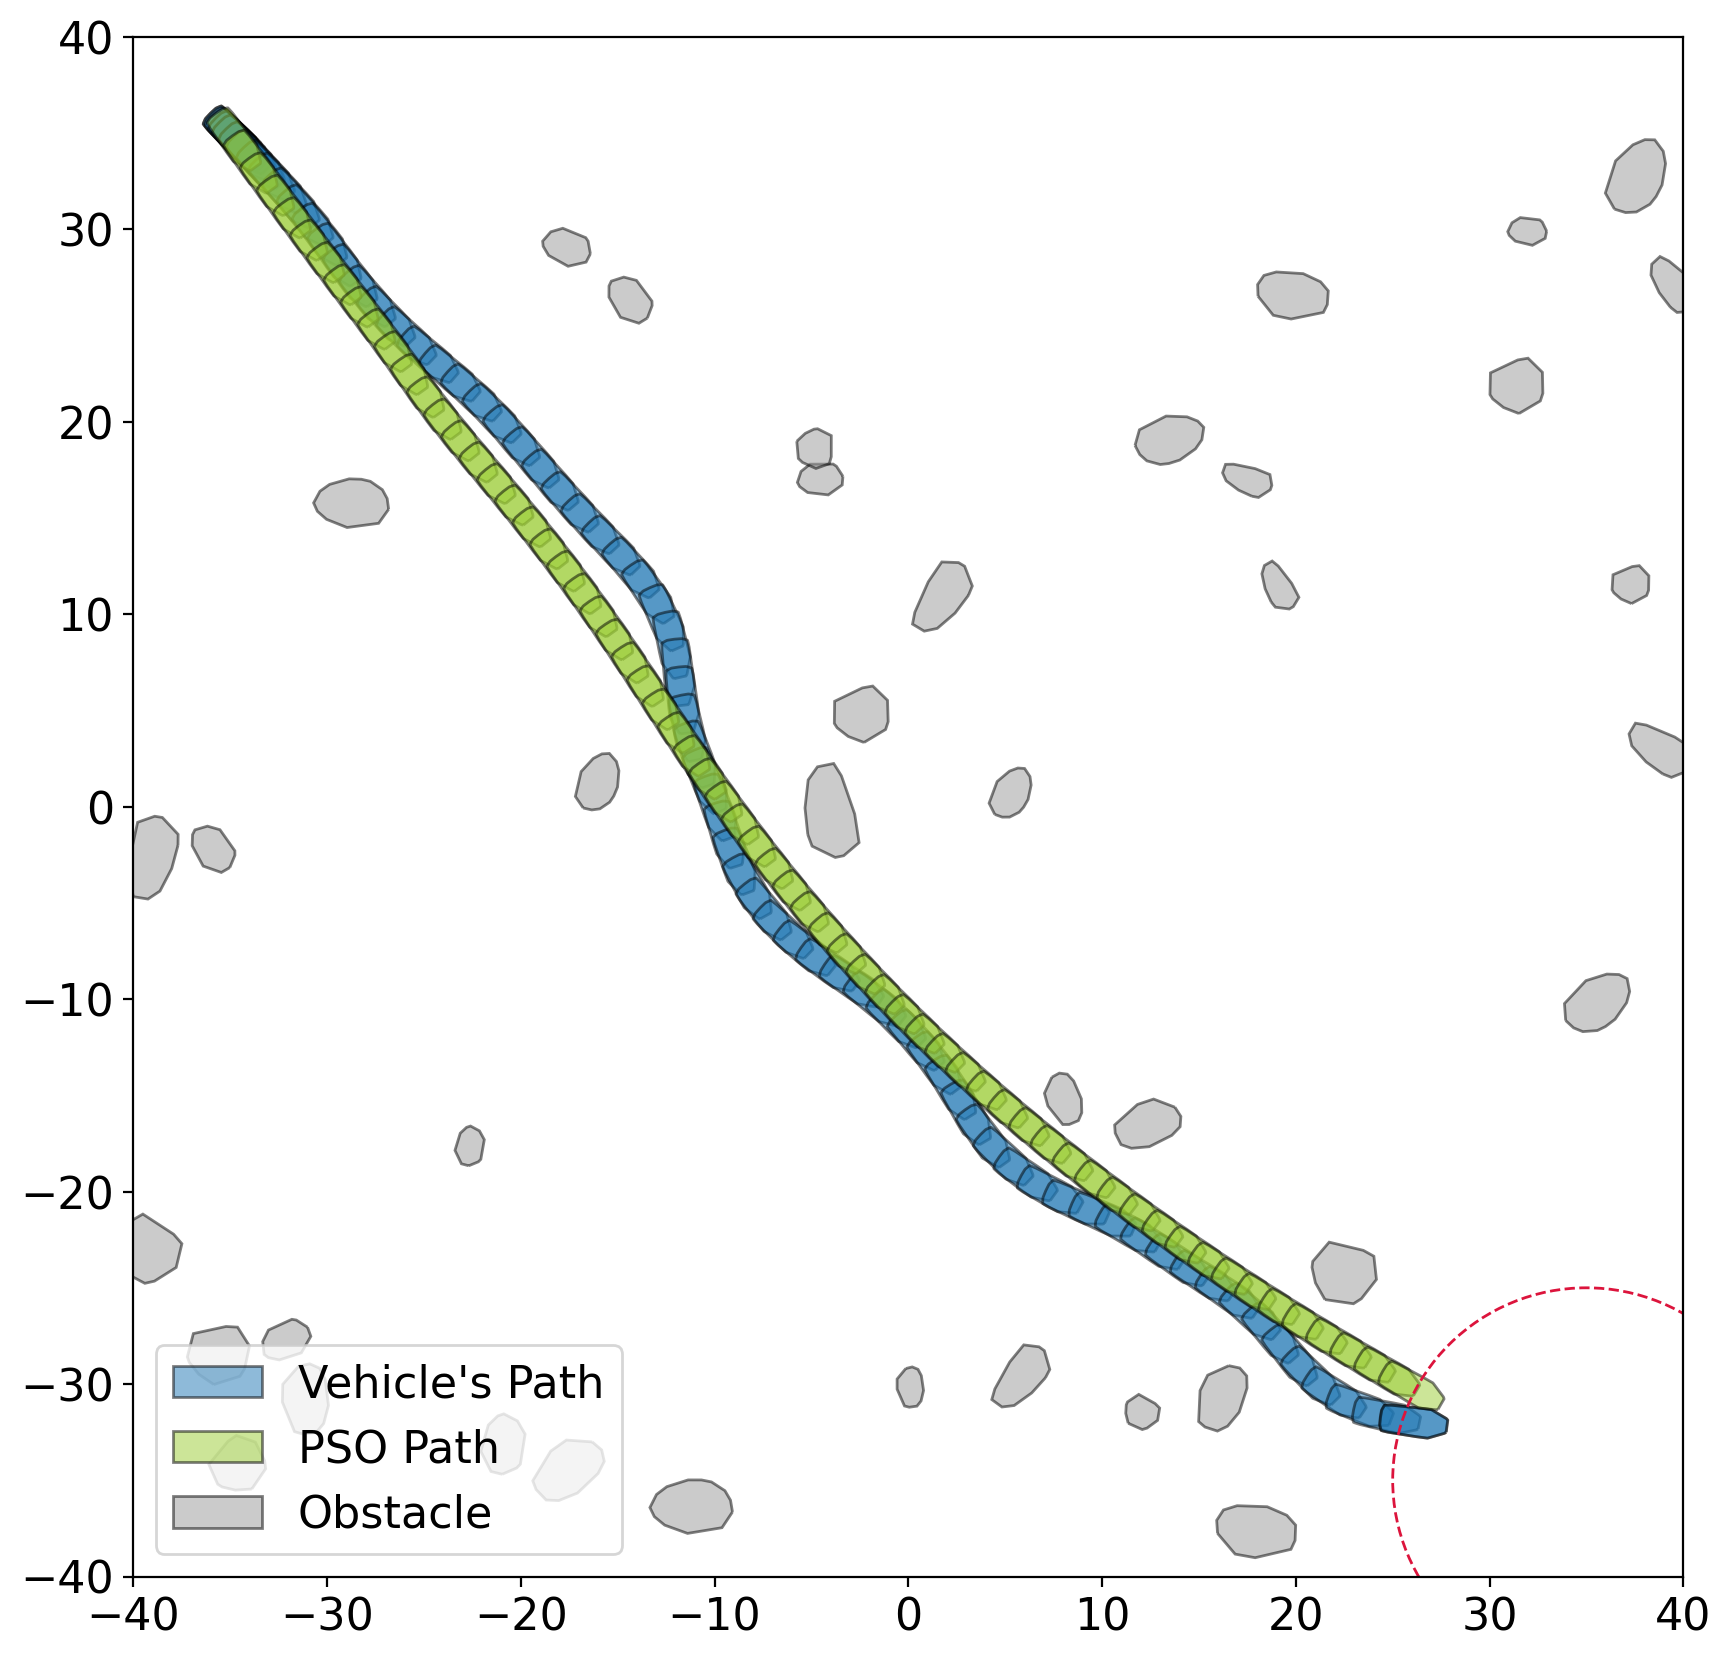
\includegraphics[height=.155\paperheight]{images/demonstration/rigid_flat_pso_example3.png}
        \caption{Example comparison between the Gator's path and PSO path.}
        \label{fig:rigid_flat_pso_example3}
    \end{subfigure}
    \hfill
    \begin{subfigure}{0.329\textwidth}
        \centering
        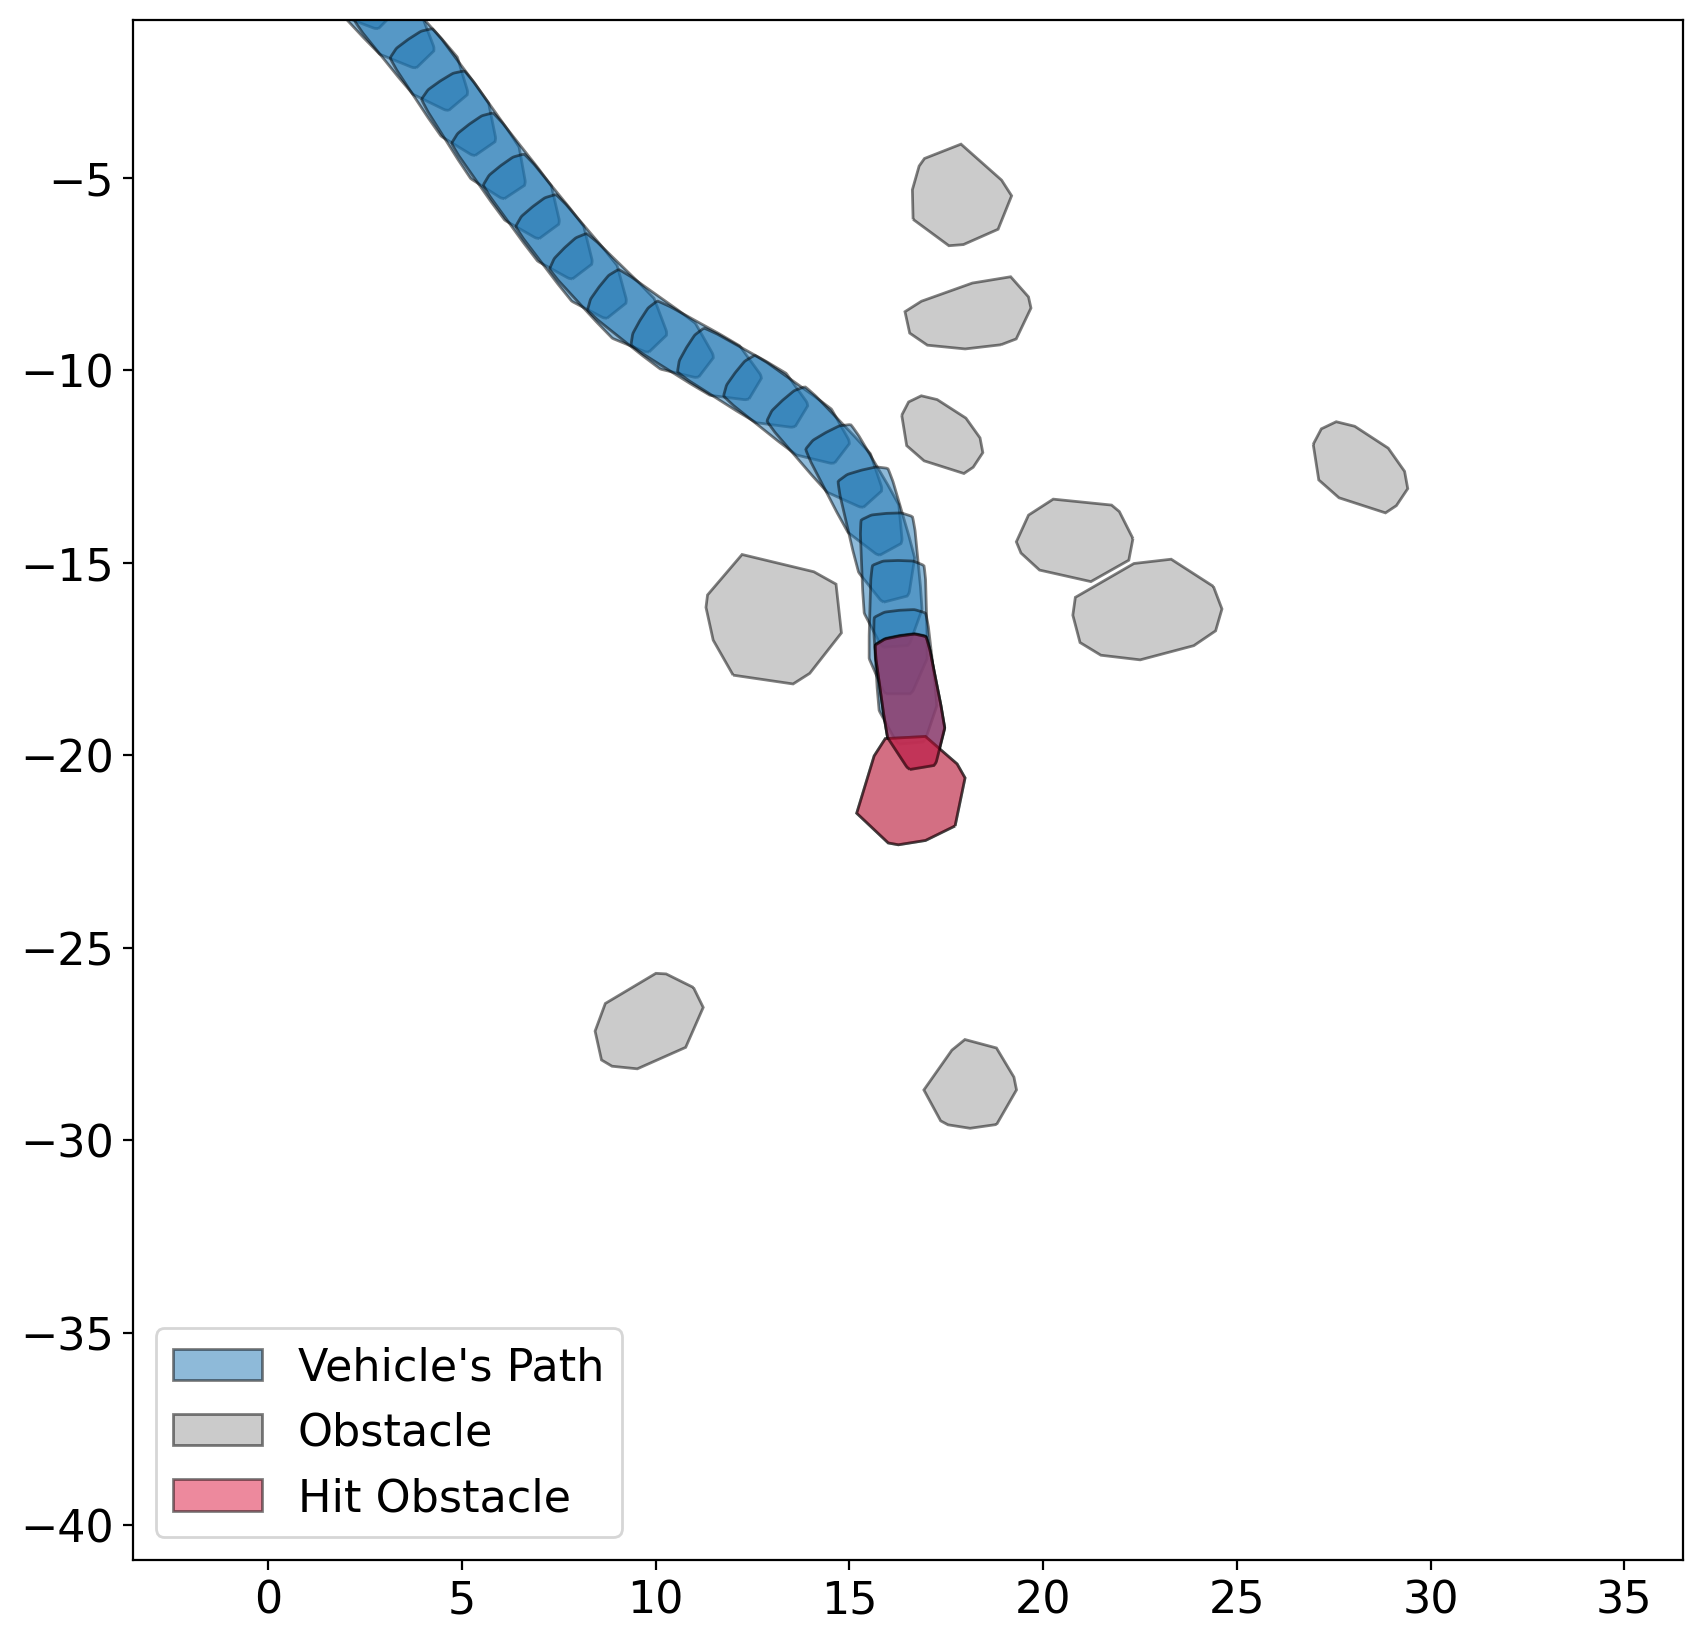
\includegraphics[height=.155\paperheight]{images/demonstration/rigid_40_failure_100.png}
        \caption{Example collision where the directness of the impacts was 100\%.}
        \label{fig:rigid_40_failure_100}
    \end{subfigure}
    \hfill
    \begin{subfigure}{0.329\textwidth}
        \centering
        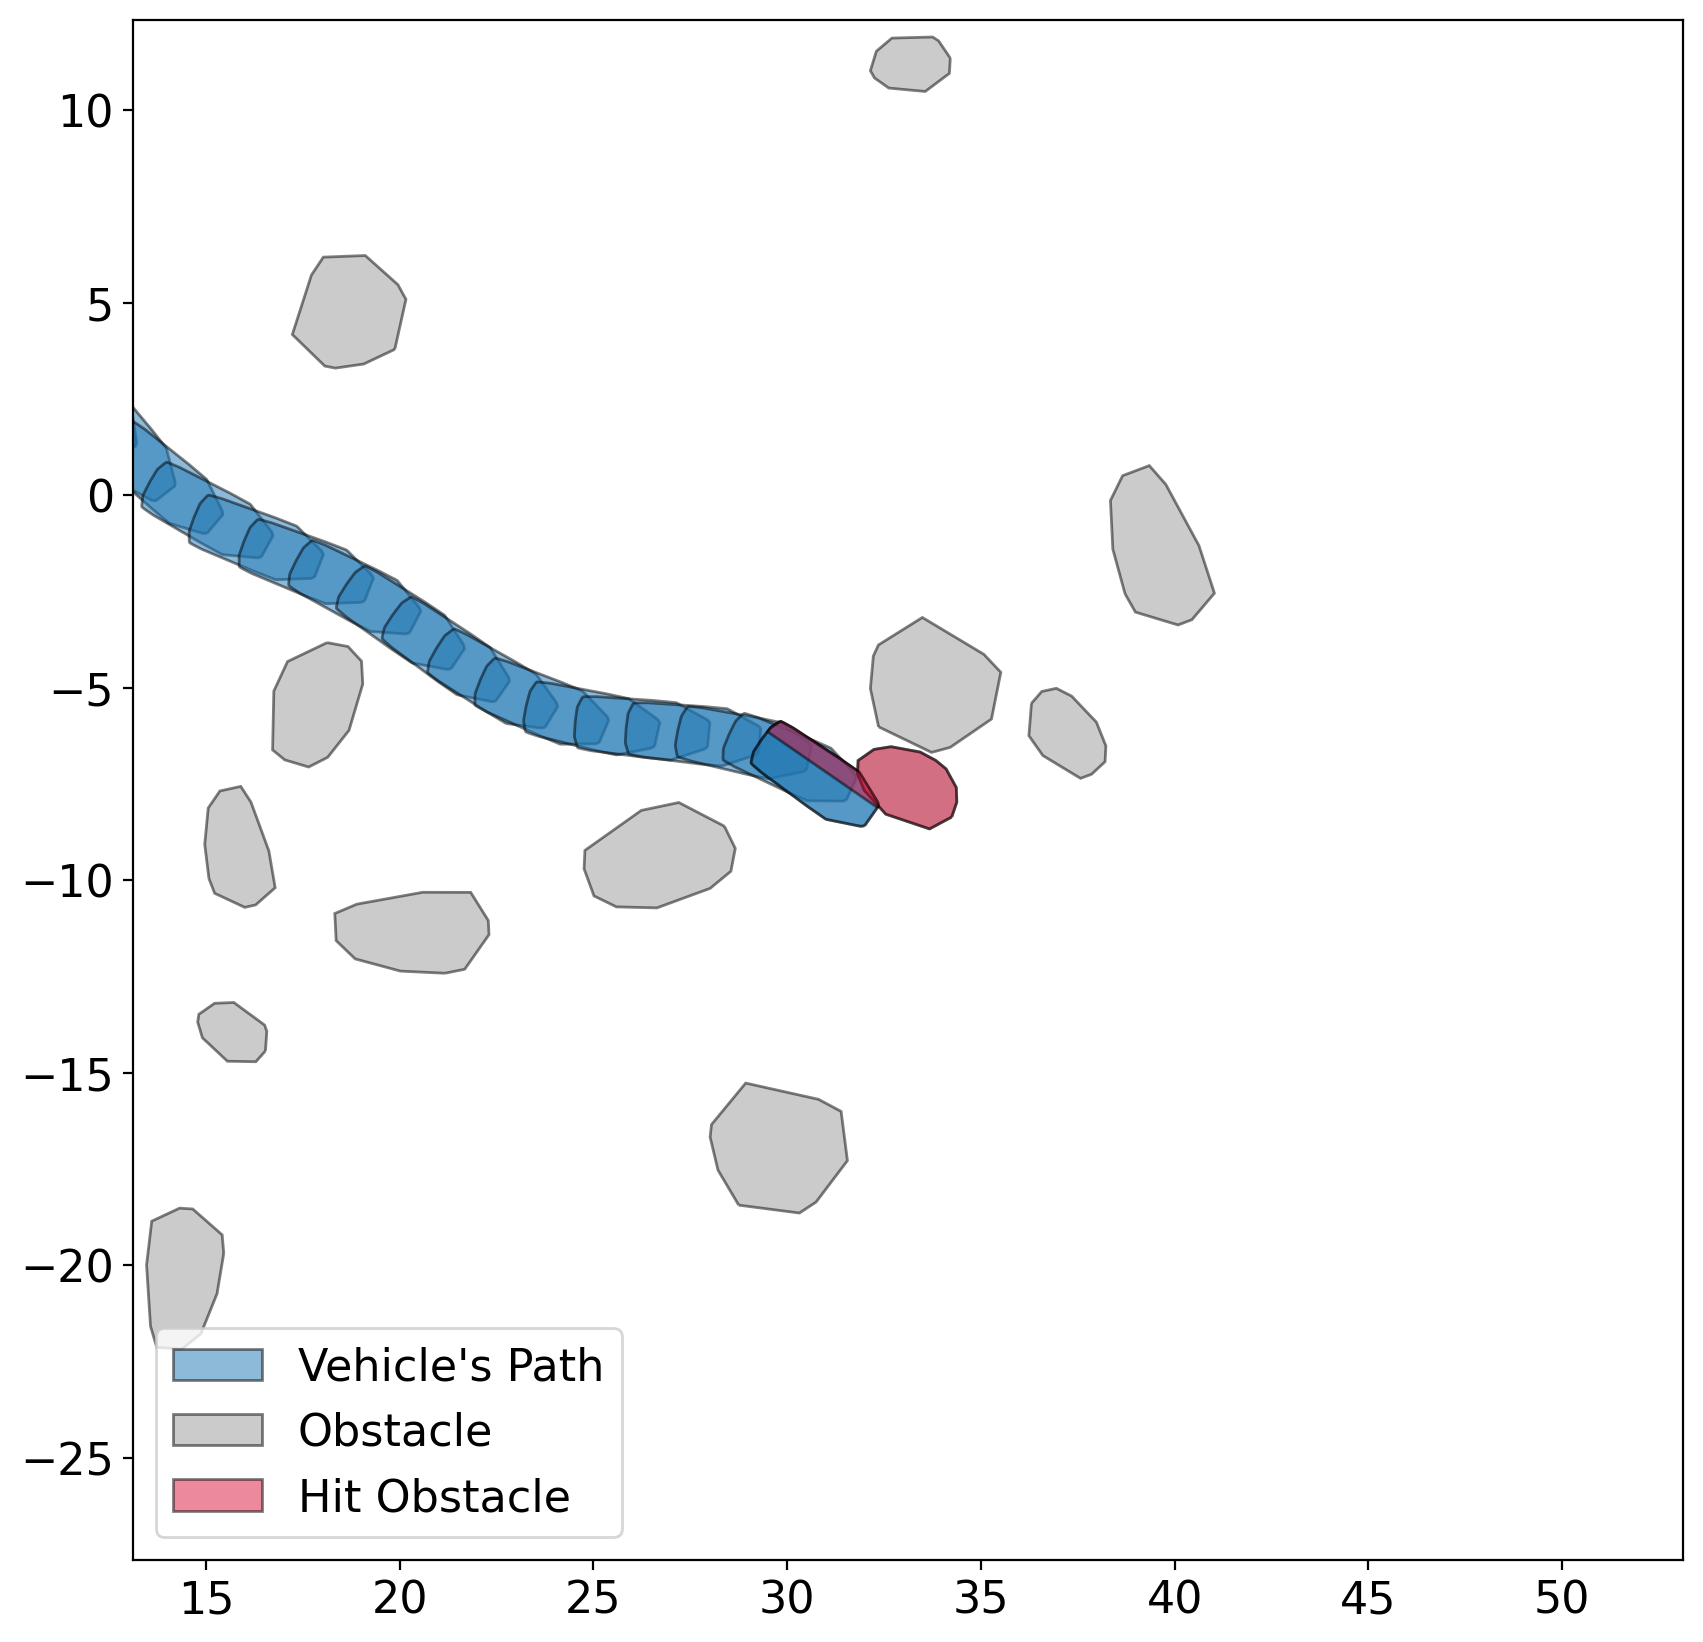
\includegraphics[height=.155\paperheight]{images/demonstration/rigid_40_failure_34.png}
        \caption{Example collision where the directness of the impacts was 34\%.}
        \label{fig:rigid_40_failure_34}
    \end{subfigure}
    \caption{Example paths showing comparison with global path planner and two levels of collision directness.}
\end{figure}

